%! TeX program = lualatex

\documentclass{fit-teorsem}

%-------------------------------------------------------------------------------
%                 Fill in seminar information
%-------------------------------------------------------------------------------
\lecturername{Ondřej Kvapil}
\lectureremail{kvapiond@fit.cvut.cz}
\papertitle{The Complexity of Interaction}
\paperauthors{Stéphane Gimenez, Georg Moser}
\paperlink{https://arxiv.org/abs/1511.01838}

%-------------------------------------------------------------------------------
%                 Use custom packages
%-------------------------------------------------------------------------------
\usepackage{enumitem}
\usepackage{amsmath}
\usepackage{amsfonts}
\usepackage{tikz}
\usetikzlibrary{arrows,cd,positioning,shapes,fit}
\usepackage{graphicx}
\graphicspath{ {./images/} }
\usepackage{caption}

\tikzset{
	encircle/.style = {draw, circle, inner sep = 0.5mm, color = red},
	dot/.style = {circle, minimum size = 1mm, inner sep = 0mm, draw = black},
	reflexive dot/.style={loop,looseness=17,in=130,out=50},
	reflexive above/.style={->,loop,looseness=7,in=120,out=60},
	reflexive below/.style={->,loop,looseness=7,in=240,out=300},
	reflexive left/.style={->,loop,looseness=7,in=150,out=210},
	reflexive right/.style={->,loop,looseness=7,in=30,out=330}
}

\begin{document}
%-------------------------------------------------------------------------------
%                 Print seminar header
%-------------------------------------------------------------------------------
\maketsheader
%-------------------------------------------------------------------------------
%                 Create your content!
%-------------------------------------------------------------------------------
\thispagestyle{empty}

\section*{Images}
\begin{minipage}{.5\textwidth}
	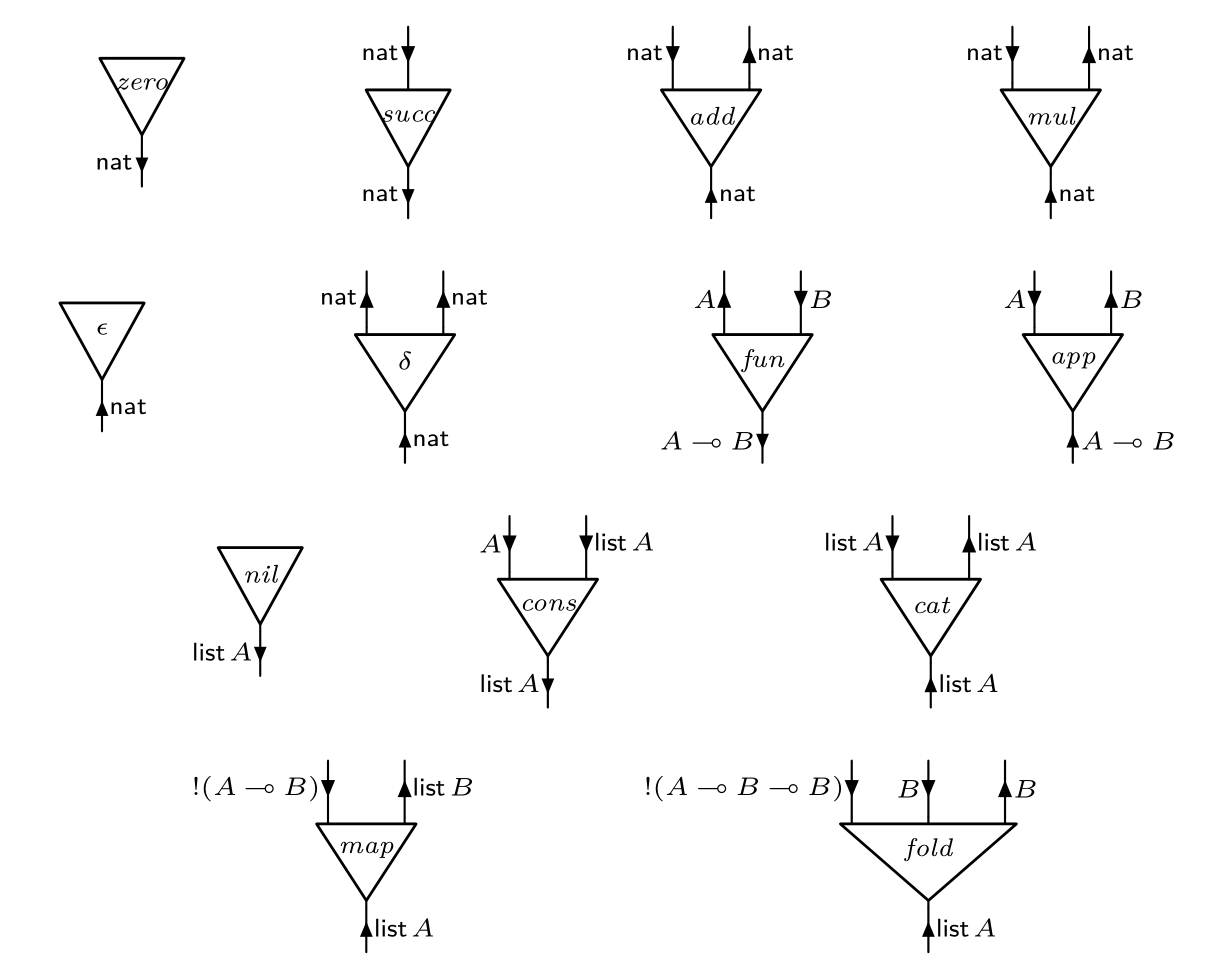
\includegraphics[width=0.95\textwidth]{inet-nodes}
	\captionof{figure}{The nodes of the interaction net system.}
	\label{fig:inet-nodes}
\end{minipage} %
\begin{minipage}{.5\textwidth}
	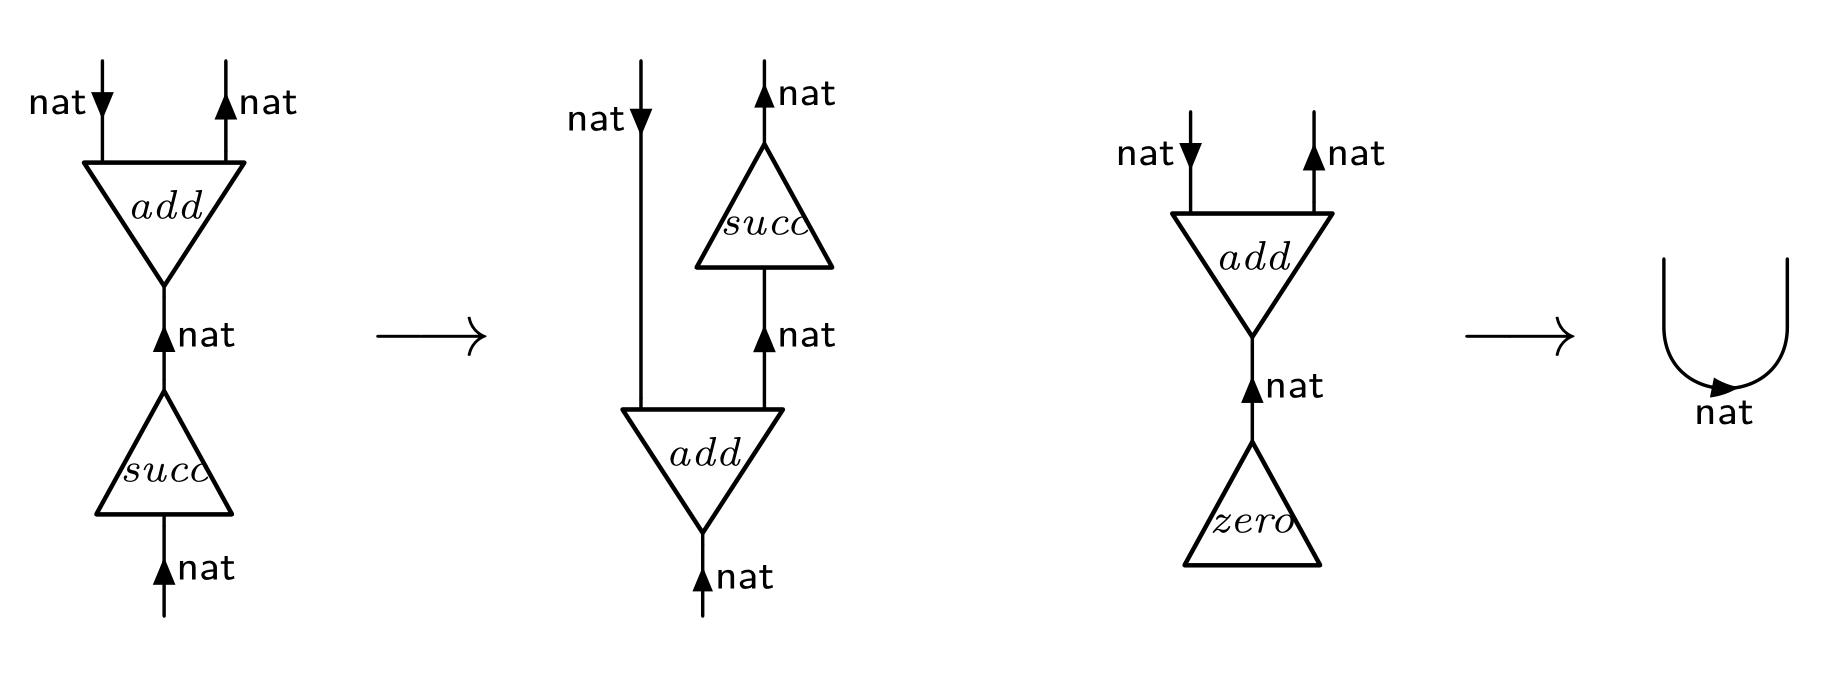
\includegraphics[width=0.95\textwidth]{inet-addition}
	\captionof{figure}{Addition of natural numbers in an interaction net.}
	\label{fig:inet-addition}
\end{minipage}

\section*{Definitions}
\begin{enumerate}
\item The \textbf{sequential convolution} of functions $f$ and $g$ is defined as
	$(f \ast g)(t) = \max_{u + v = t} f(u) + g(v)$.

\item The \textbf{generalised sequential convolution} of a family of functions $\{f_i\}_{i \in I}$ is
	defined as \[
		\left(\coprod_{i \in I} f_i\right)(t) = \max_{\sum_{i \in I} t_i = t} \sum_{i \in I} f_i(t_i)
	.\]

\item \textbf{Cost Model} Given a timed reduction $\longrightarrow$ and a notion of space
	occupation $|\cdot|$ for nets (typically, the number of nodes) in a chosen
	space domain $S$, we say that $N$ admits:
	\begin{itemize}
		\item $\tau \in T$ as a time bound if whenever
			$N \stackrel{t}{\longrightarrow} M$, $t \le \tau$
		\item $\sigma \in S$ as a space bound if whenever
			$N \stackrel{t}{\longrightarrow} M$, $|M| \le \sigma$
		\item $\gamma : T \to S$ as a space-time bound if whenever
			$N \stackrel{t}{\longrightarrow} M$, $|M| \le \gamma(t).$
	\end{itemize}
\end{enumerate}

\section*{Theorems}
\textbf{Theorem 1} (Sequential Space-Time Complexity) Associate a function $\gamma_c : T \to S$,
called \textit{space-time potential}, to every typed node $c$, such that
$\underbrace{\gamma_c(0) \ge |c|}_{\begin{subarray}{c}
	\text{The space complexity} \\
	\text{of node $c$ at time $0$ is at least} \\
	\text{the space weight of node $c$}
\end{subarray}}$ and \[
	\underbrace{\overbrace{\left(\coprod_{c \in L} \gamma_c\right)}^{\begin{subarray}{c}
			\text{The convolution} \\
			\text{on the LHS}
		\end{subarray}}\overbrace{(t + d)}^{\begin{subarray}{c}
			\text{at a time $t$ offset} \\
			\text{by the duration $d$} \\
			\text{of the reduction rule}
		\end{subarray}}}_{
	\begin{subarray}{c}
		\text{The maximum space complexity} \\
		\text{of the LHS at time $t + d$}
	\end{subarray}}
		\ge \underbrace{\overbrace{\left(\coprod_{c \in R} \gamma_c\right)}^{\begin{subarray}{c}
				\text{The convolution} \\
				\text{on the RHS}
			\end{subarray}}(t)}_{
		\begin{subarray}{c}
			\text{The maximum space complexity} \\
			\text{of the RHS at time $t$}
		\end{subarray}}
\] for every reduction rule $L \stackrel{d}{\longrightarrow} R$. Then \[
	N \stackrel{t}{\longrightarrow}_s M
		\Longrightarrow |M| \le \left(\coprod_{c \in N} \gamma_c\right)(t)
.\]

\textbf{Corollary 2} (Sequential Time Complexity) Associate $\tau_c \ge 0$, called \textit{time potential},
to every typed node $c$, such that $\sum_{c \in L} \tau_c \ge \sum_{c \in R} \tau_c + d$ for
every reduction rule $L \stackrel{d}{\longrightarrow} R$. Whenever
$N \stackrel{t}{\longrightarrow}_s M$: \[
	t \le \sum_{c \in N} \tau_c
.\]

\textbf{Corollary 3} (Sequential Space Complexity) Associate $\sigma_c \ge 0$, called
\textit{space potential}, to every typed node~$c$, such that
$\sum_{c \in L} \sigma_c \ge \sum_{c \in R} \sigma_c$
for every reduction rule $L \stackrel{d}{\longrightarrow} R$. Whenever
$N \stackrel{t}{\longrightarrow}_s M$: \[
	|M| \le \sum_{c \in N} \sigma_c
.\] 

\textbf{Theorem 2} (Parallel Space-Time Complexity) Associate a function $\overline{\gamma}_c : T \to S$,
called \textit{parallel space-time potential}, to every schedule-typed node $c$, such that
$\overline{\gamma}_c(0) \ge |c|,$ $\overline{\gamma}_{[c]^d}(t + d) \ge \overline{\gamma}_c(t),$
and $(\sum_{c \in L} \overline{\gamma}_c)(t + d) \ge (\sum_{c \in R} \overline{\gamma}_c)(t)$ for
every reduction rule $L \stackrel{d}{\longrightarrow} R$. Whenever
$N \stackrel{t}{\longrightarrow}_p M$: \[
	|M| \le \left( \sum_{c \in N} \overline{\gamma}_c \right)(t)
.\]

\textbf{Corollary 4} (Parallel Time Complexity) Associate $\overline{\tau}_c \ge 0$, called
\textit{parallel time potential}, to every schedule-typed node $c$, such that
$\overline{\tau}_{[c]^d} \ge \overline{\tau}_c + d$ and
$\max_{c \in L} \overline{\tau}_c \ge \max_{c \in R} \overline{\tau}_c + d$ for every reduction rule
$L \stackrel{d}{\longrightarrow} R$. Whenever $N \stackrel{t}{\longrightarrow}_p M$: \[
t \le \max_{c \in N} \overline{\tau}_c
.\]
\end{document}
